\documentclass[a4paper,11pt]{article}
\usepackage[utf8]{inputenc}
\usepackage[italian]{babel}
\usepackage{graphicx}
\usepackage[colorlinks=true,linkcolor=blue]{hyperref}
\graphicspath{ {../app/src/main/res/mipmap-xxxhdpi/} {./images/}}

\title{Simulatore di scherma per Android\\con riconoscimento di gestures}
\author{Francesco Bultrini, matricola 278696\\
 Claudio Pannacci, matricola 283526}
\date{Anno accademico 2016-2017}

\begin{document}

\begin{figure}[t]

  \centering
  
\includegraphics{img_fency_logo}

\end{figure}

\maketitle
\newpage

\tableofcontents
\newpage

\subsection{Abstract}
L'obiettivo di questo progetto è la realizzazione di un gioco  ispirato allo sport della scherma, per cellulari dotati di sistema operativo Android che, nella sua versione finale, consisterà in una sfida locale tra due giocatori dove lo scambio di informazioni avverrà tramite Bluetooth. Si valuta anche la possibilità di utilizzare la tecnologia NFC per eseguire il \hyperref[pairing]{\emph{pairing}} dei dispositivi.\\
\subsection{Realizzazione}
Si è deciso di utilizzare il \hyperref[spirale]{\emph{modello a spirale}} come modello di sviluppo e ad ogni ciclo verrà realizzato un prototipo. Non tutte le funzionalità saranno presenti da subito ma verranno implementate in \hyperref[release]{\emph{release}} successive. \\Per la codifica è stato adottato il metodo del \hyperref[pairp]{\emph{Pair Programming}} utilizzando \href{https://developer.android.com/studio/index.html}{Android Studio} come ambiente di sviluppo.\\Il codice sorgente è pubblicato su GitHub all'indirizzo: \begin{center}
\url{https://github.com/Disorganizzazione/Fency}\\
{\footnotesize Il codice sorgente è coperto da licenza GNU.}
\end{center}
\newpage

\part{Riconoscimento delle gestures e modalità allenamento}
\ 
\section{Analisi dei requisiti}
\subsection{Requisiti riconoscimento gesture}
Al fine di riconoscere le \hyperref[gesture]{\emph{gestures}} si deve accedere, tramite classi di sistema, ai valori di accelerometro, giroscopio e magnetometro. Per ridurre il dominio dei movimenti da analizzare, sarà necessario definire un orientamento del telefono (in direzione orizzontale, con lo schermo rivolto verso l'alto) e assicurarsi che tale stato venga mantenuto durante lo spostamento.\\ A questo scopo la classe \textbf{SensorFusion} di Paul Lawitzki, che combina i dati del giroscopio a quelli del magnetometro riducendo il rumore, permette di avere informazioni affidabili sull'orientamento del dispositivo tramite i valori di \hyperref[pra]{\emph{pitch}}, \hyperref[pra]{\emph{roll}} e \hyperref[pra]{\emph{azimuth}}. La descrizione dell'affondo si basa sui dati forniti dall'accelerometro e, utilizzando la modalità \textbf{Linear Acceleration}, si hanno i valori di accelerazione sui tre assi, senza la componente gravitazionale. Il movimento dell'affondo causa un'accelerazione positiva sull'asse Y (parallelo al lato lungo del dispositivo) seguito da una accelerazione di modulo maggiore, stesso verso e direzione opposta, dovuta all'arresto del dispositivo nel momento in cui si conclude l'affondo. Inoltre, per impedire ad altri movimenti (come lo scuotimento) di essere classificati come affondi bisogna accertarsi dell'effettivo spostamento del dispositivo. Non basta quindi impostare una soglia minima di accelerazione ma è necessario anche stimare la durata del movimento.
\subsection{Requisiti modalità allenamento}
\newpage

\section{Struttura del codice}
\subsection{Diagramma di classe}
\noindent\makebox[\textwidth]{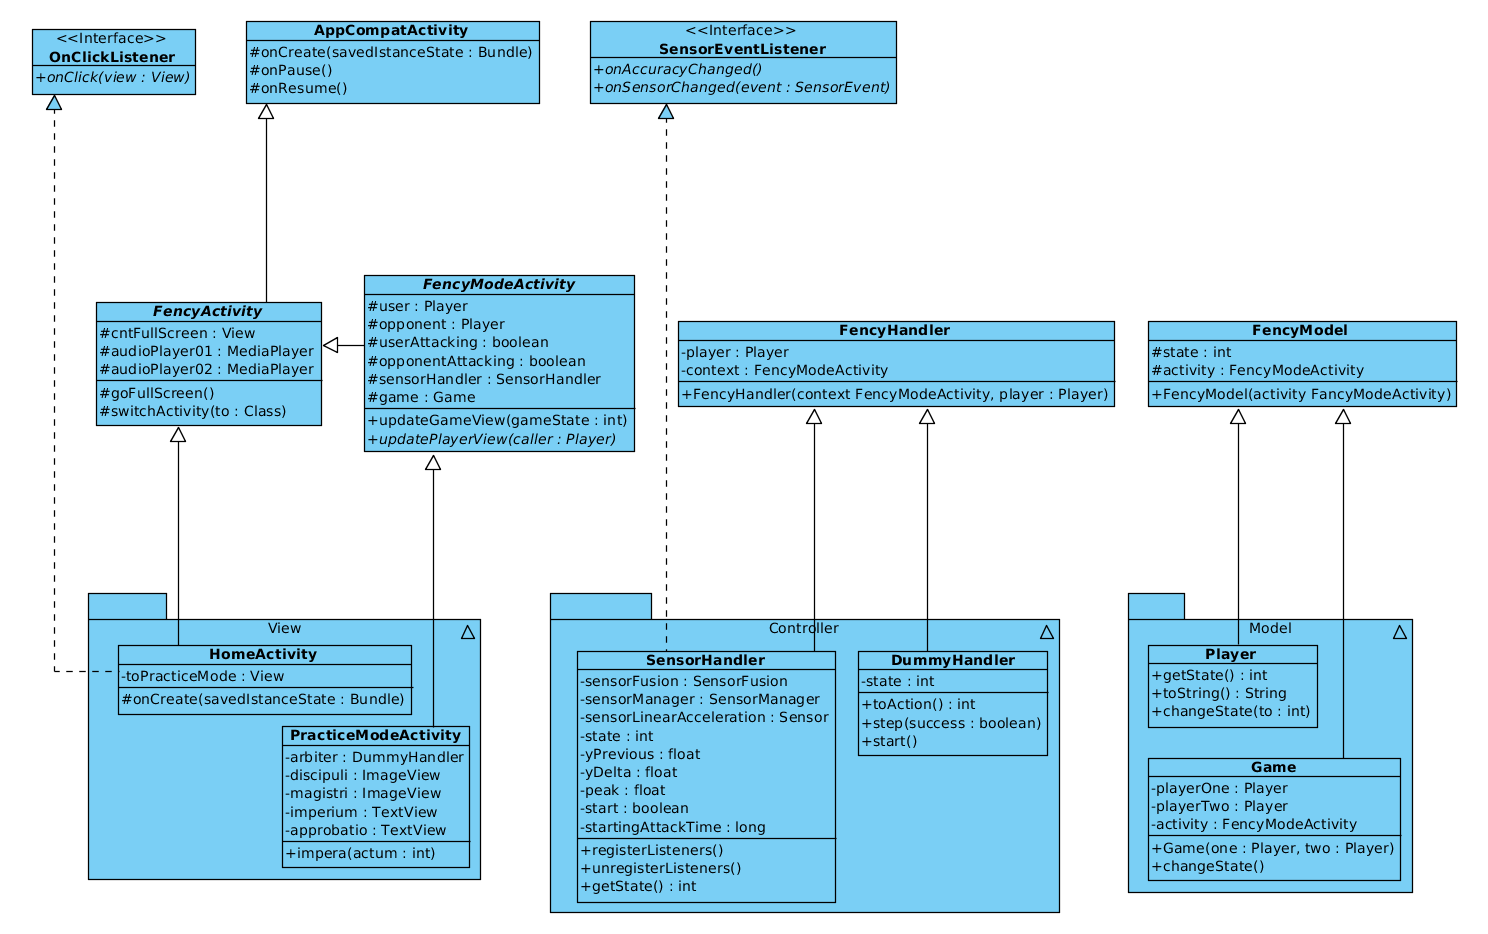
\includegraphics[width=\paperwidth]{UML_classes}}
\subsection{Design pattern}
Come mostrato nel diagramma, abbiamo applicato una variante del design pattern \hyperref[MVC]{\emph{Model View Controller}} nella quale il controller dei modelli giocatore (\textbf{SensorHandler}) ne modifica lo stato in base ai valori dei sensori anzi che in risposta ad un' interazione con le loro componenti grafiche da parte dell'utente. Ogni volta che lo stato del modello cambia, esso chiama la funzione \emph{updatePlayerView()} che ne aggiorna la visualizzazione.
\newpage

\subsection{Diagrammi di sequenza e di stato}
\subsubsection{Cambiamento dello stato del giocatore}
\noindent\makebox[\textwidth]{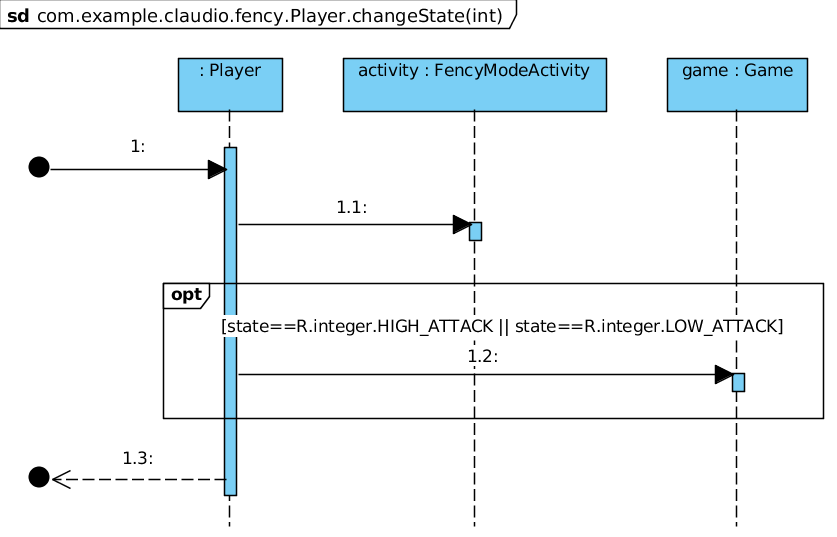
\includegraphics[scale=0.4]{PlayerChangeState} \ \ \ \ \ \ \ \ 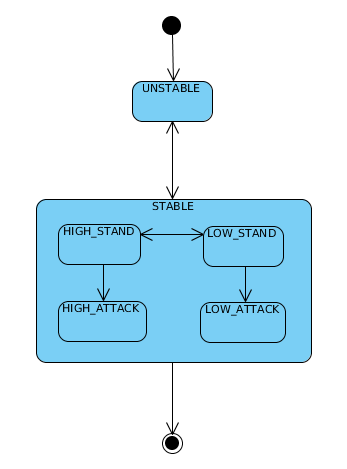
\includegraphics[scale=0.42]{PlayerStates}}\\Ogni volta che un giocatore passa ad uno stato di attacco, il \textbf{Player Model} chiama la funzione \emph{ChangeState()} del \textbf{Game Model}...
\subsubsection{Cambiamento dello stato di gioco}
\noindent\makebox[\textwidth]{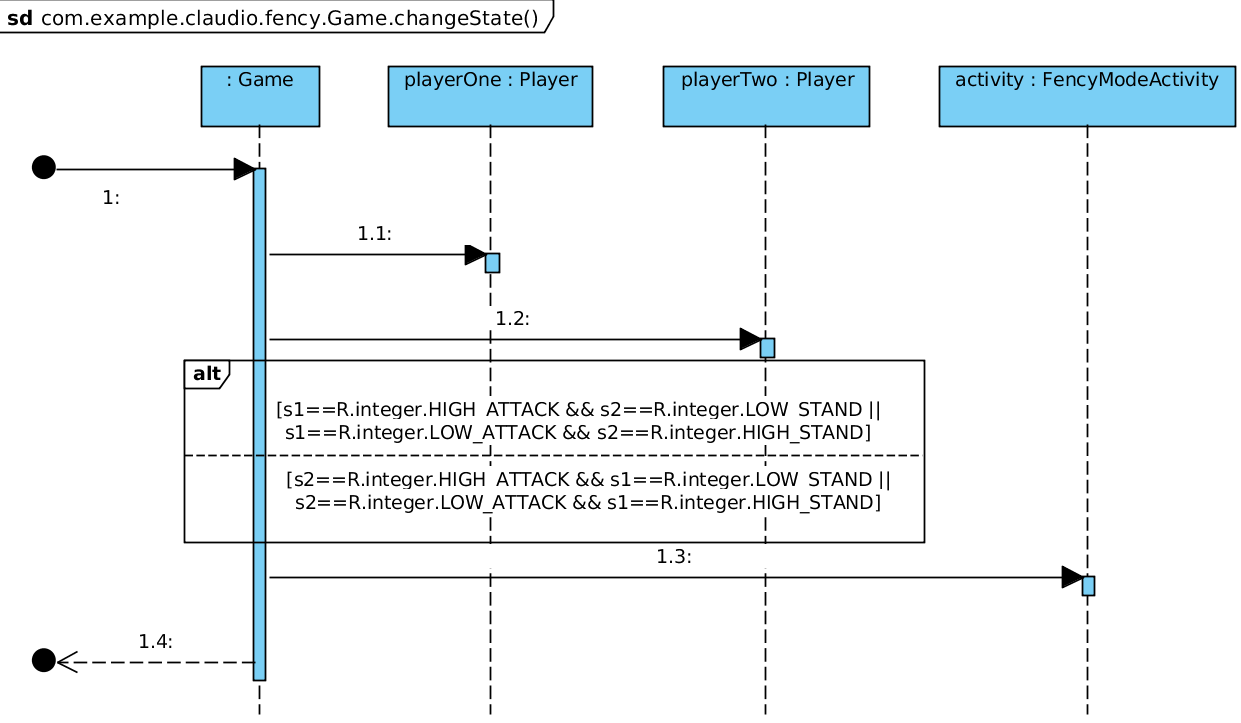
\includegraphics[scale=0.3]{GameChangeState}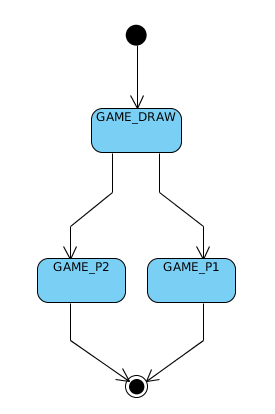
\includegraphics[scale=0.5]{GameStates}}\\...che controlla gli stati di entrambi i giocatori.
\newpage

\section{Meccaniche di gioco}
\subsection{Casi d'uso}
\noindent\makebox[\textwidth]{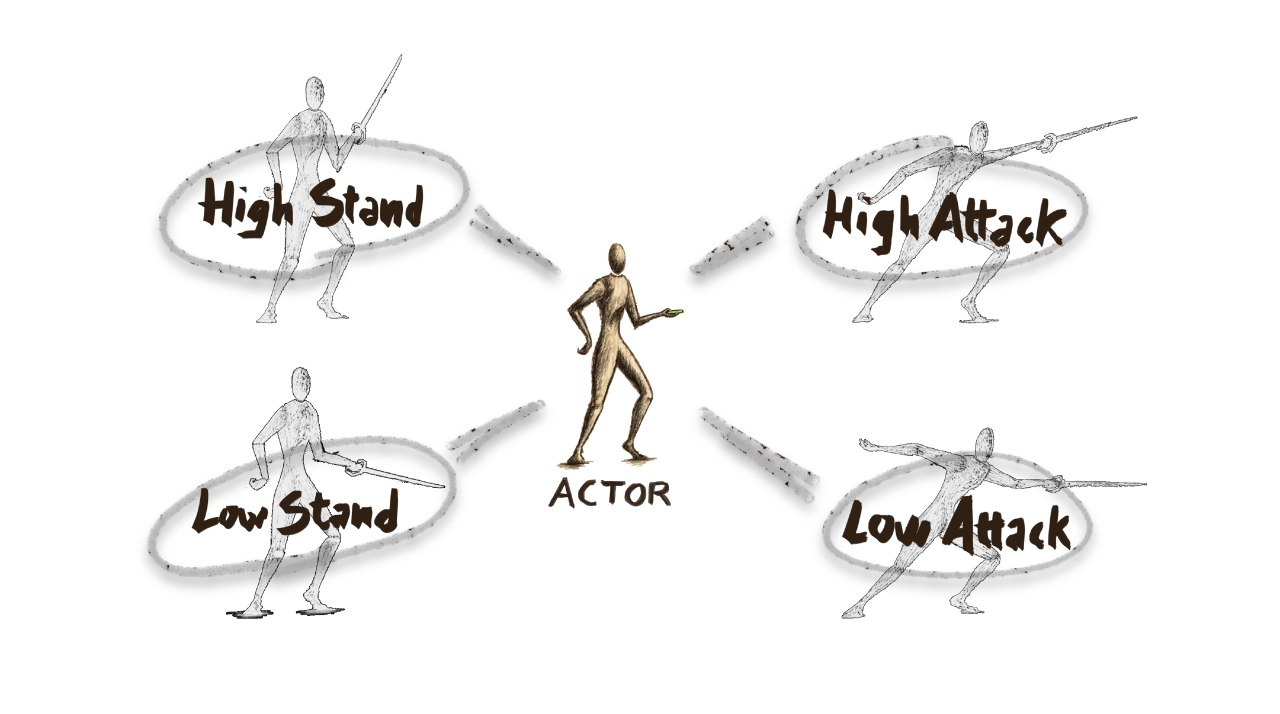
\includegraphics[width=\paperwidth]{UseCases}}
\subsection{Bho}
Il giocatore bla bla

\newpage

\section{SensorHandler}

\subsection{Stato}

\subsection{Attività}
\newpage

\renewcommand\thesection{}
\section{Glossario}
\ \\
\textbf{gesture}: specifico movimento del dispositivo \\ \label{gesture}\textbf{pairing}: connessione reciproca tra due dispositivi\\ \label{pairing}\textbf{release}: rilascio del software\\ \label{release}\textbf{Pitch, Roll, Azimuth}: (come in figura)\\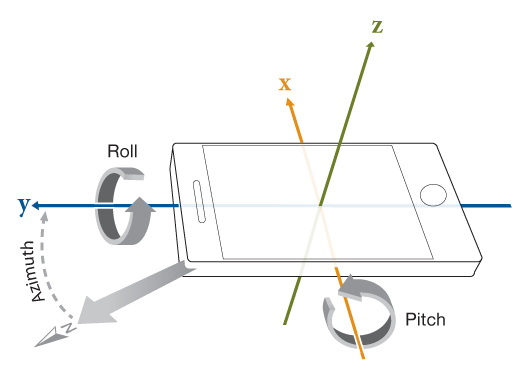
\includegraphics[scale=0.5]{PitchRollAzimuth}\\ \label{pra}\textbf{Modello a spirale}: modello di cilco di vita del software proposto da Barry Boehm nel 1988 \\ \label{spirale}\url{https://it.wikipedia.org/wiki/Modello_a_spirale}\\\textbf{Pair programming}: tecnica di sviluppo del software nella quale due programmatori lavorano insieme a una postazione di lavoro \\ \label{pairp}\url{https://it.wikipedia.org/wiki/Pair_programming}\\\textbf{Model View Controller (MVD)}: è un pattern architetturale molto diffuso nello sviluppo di sistemi software ad oggetti che separa la logica di visualizzazione di un oggetto da quella di gestione.\\ \label{MVC}\url{https://it.wikipedia.org/wiki/Model-View-Controller}

  


\end{document}